\section{Influence Propogation}

 Influence propogation algorithms attempt to model the spread of ideas (Rogers 2003), viruses (Anderson and May 1991), word-of-mouth recommendations (Goldenberg, Libai and Muller 2001), viral marketing campaigns (Kempe, Kleinberg and Tardos 2003) or other transmissable entities, through a social network.

Influence propogation algorithms make the following assumptions about the social networks that they model. Social networks are modelled as directed graphs, with nodes representing individuals, and vertices representing relationships between individuals. In most influence propogation models, nodes can be in one of two states: "converted" or "unconverted". At the begin of the simulation, a subset of the nodes will be converted; over time they will convert their unconverted neighbours. There is an assumption of monotonicity, ie, converted nodes do not become unconverted.

 The exact conditions that determine when nodes will change from unconverted to converted depends on the influence propogation model used. There are three main models of transmission used; the independent cascade model, the linear threshold model, and ???

Mention more complicated models, three states etc

\subsection{Independent Cascade}
 In the independent cascade model, whenever a node becomes converted, it has one chance to convert each of its neighbours. Every edge (A -> B) is assigned a weight between 0 and 1, which represents the probability that node A can convert node B, or vice versa.

Assume a node n has a set of x neighbours n\_0,n\_1,n\_2...n\_x each with edge weights e\_0,e\_1,e\_2...e+x. When n is converted, each neighbour n\_m has a e\_m chance to become converted.

This can be expressed in pseudocode as follows:

\begin{verbatim}
recently-converted-nodes = a queue of the initially converted nodes
while recently-converted-nodes is non-empty {
  node = recently-converted-nodes.next()
  for each neighbour in node.neighbours {
    if rand(0,1) < neighbour.edge-weight {
      neighbour.converted = true
      recently-converted-nodes.enqueue(neighbour)
    }
  }
}
\end{verbatim}

\subsection{Linear Threshold}
 In the linear threshold model, every node has a threshold value t. When the number of converted neighbours is greater than t, the node becomes converted. Again, edges can be weighted, in which case the condition for conversion is:

Maths: sum for all neighbours(if neighbour is converted(0,1) * edge weight)

That is, nodes are converted when a threshold of their neighbours are converted. In pseudocode:

\begin{verbatim}
do {
  changed-nodes = 0
  for each node in unconverted-nodes {
    neighbour-influence = 0
    for each neighbour in neighbours {
      if neighbour.converted {
        neighbour-influence += neighbour.edge-weight
      }
    }
    if neighbour-influence >= node.threshold {
      node.converted = true
      changed-nodes += 1
    } 
  }
} while changed-nodes > 0
\end{verbatim}

\subsection{Decreasing Cascade Model}

The decreasing cascade model fits situations where nodes are less likely to be influenced with each conversion attempt. One real world example was [cite:digg], where it was found that a standard independent cascade model did not fit the spread of stories through the social news site Digg. The decreasing cascade model proved to be a much better fit for the data; one possible conclusion from this is that if users do not ``digg'' (vote for) a story the first time they are exposed to it, they are unlikely to do so on subsequent exposures.

The decreasing cascade model works similarly to the independent cascade model, but after a failed conversion attempt, the unconverted node becomes more difficult to convert in future. In the most basic example, the probability of future conversions becomes 0 after 1 failed conversion attempt.

\subsection{Influence Maximisation Problem}

[Maximizing the Spread of Influence through a Social Network]

[http://arxiv.org/pdf/math/0612046.pdf]

One common use of an influence propogation model is to determine the best subset of nodes, that, if converted at the start of the simulation, will maximise the number of converted nodes at the end of the simulation. More formally, given a fixed budget k, and a function f(S), which takes an initial set of converted nodes and computes the expected final number of converted nodes, find a set of k nodes that maximises f(S).

One practical example would be a viral marketing company that might wish to kickstart their campaign by giving a group of influential bloggers a free trial of their service, and hope that these bloggers would then hopefuly recommend the product to their followers, who would recommend it to their followers, and so on. One strategy for choosing the optimal set of free trial users would be to rank the bloggers by a precomputed influence rating, and then select the top k most influential individuals from the list.

Even if influence of a single node could be computed reliably, this strategy would not generally find the optimum subset. For example, the most influential bloggers might share the same audience, wheras a less popular blogger might have considerable influence amongst a niche audience. In graph theory terms, there may be a short distance between two influential nodes -- they may even share overlapping neighbourhoods -- which means there may be a set of nodes far from the influential pair. These nodes might be more influenced by a node that is less globally influential, but nearer. Obviously, the structure of the graph determines the likelihood of this. For example, graphs with a community structure are more likely to require an influential seed node within each community to achieve maximum influence.

Solving the optimum problem is NP-hard, for both the linear threshold and independent cascade models. This can be shown by reducing the independent cascade maxmisation problem to a special case of the set cover problem, and the linear threshold maximisation problem to a special case of the vertex cover problem.

However, a greedy solution works as an approximation. !he set of nodes chosen by the greedy solution will convert at least 63\% of the nodes converted by the optimum solution. This result can be proved by showing that the function f(S) is monotonic and submodular.

The monotonicity property requires that f(S) increases whenever an element is added to S; ie, f(S+v) >= f(S) for any S, v. Proving this property of f(S) is trivial. The submodularity property can be intuitively thought of as a ``dimininishing returns'' property; if S is a subset of T, the marginal gain from adding an element v to S is at least as high as adding the same element to T. Formally:

f(S+v) - f(S) >= f(T+v) - f(T)

Nemhauser, Wolsey and Fisher showed that a greedy-hill climbing algorithm can be used to find the optimum value of such a submodular function to within a factor of 1/(1-e), or ~63\%. The greedy algorithm works by adding elements to the seed set one at a time, each time choosing the element that provides the largest marginal increase to the value of the function. In the case of influence maximisation, this is the node that adds the greatest number of converted nodes at the end of the simulation.

Of course, this method relies on a fast method of working out the expected number of nodes that will be converted by a seed set. There is currently no simple means of calculating this value, so in practice a Monte Carlo method is used; ie, running several iterations of the model and taking an average of the final number of converted nodes. This is computationally expensive, though some work has been done to improve the performance. [CITE??]

\subsection{Adversarial Social Networks}

 There are limitations to the two-state models described above. For example, they cannot represent any scenario where two competing ideas spread through a network. An alternative model for such situations allows nodes to be in one of 3 states; "unconverted", "converted to idea A", or "converted to idea B". In this case, A and B represent opposing beliefs.

The paper [Influence Propagation in Adversarial Social Network—Impact of Space and Time] looks in depth at this situation, and applies it to the spread of radical and counter-radical ideas through the Muslim community.

They observe that the key reason that the standard influence propogation model cannot capture the nature of adverserial networks is as follows. Observe the network described in fig???. Node\_2 is initially converted to idea A, and node\_4 is converted to idea B. All other nodes are unconverted. At some point, node\_9, which is a bottleneck between the two sides of the graph, may be converted to one idea or the other. Once this happens -- assume that it is converted to idea A -- there will be no chance that it will ever be converted to idea B. For that reason, there is no way that idea B can ``pass through'' node\_9 and so no way that nodes 10 to 14 will ever be converted to idea B. The standard influence models have no way to capture this situation.

\begin{figure}[htbp]
\centering
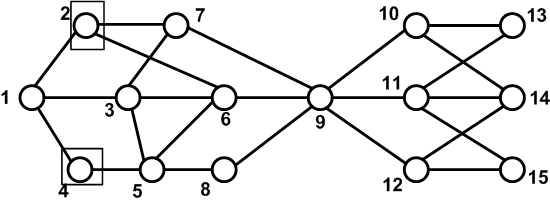
\includegraphics[width=0.5\textwidth]{./img/adversial_network.png}
\caption{Adverserial network}
\label{fig:adverserial_network}
\end{figure}

Other real-life applications of this concept include marketing -- promoting your product while a rival company is promoting a competing product -- or preventing the spread of misinformation. A recent example was the Kony 2012 campaign, a viral video spread by a non-profit activist organisation to highlight the issue of child soldiers in Uganda. The video spread very rapidly via online social networks; however, this soon led to people questioning the aims and methods of the campaigning organisation. This led to a counter-campaign that also spread virally, via social media. (Of course, which party provided misinformation in this scenario depends on individual perceptions).

[Limiting the Spread of Misinformation in Social Networks] looks more in depth at the problem of countering mis-information. They quantify this situation as a ``Multi-Campaign Independent Cascade Model'', where two campains, C and L, spread through a network. Each campaign has an initial seed set of nodes, A\_C/A\_L. As with the independent cascade model, when a node is converted, it has one chance to convert each of its neighbours. The probability that a node n converts its neighbour o is given by p\_C\_n\_o / p\_L\_n\_o, depending on which campaign the node was converted to. Note that in the general case, their may be different probabilities for the two campaigns (representing the situation where one campaign is more ``infectious'' than the other). Unlike in the independent cascade model, when an unconverted node has multiple converted neighbours, the order of ``conversion attempts'' matters; eg, campaign C may succeed in converting a node before campaign L has had the chance to convert it. Their model assumes that one campaign always precedes the other in such situations, ie, that campaign always gets the ``first chance''.

They also used a more specific model, the ``Campaign Oblivious Independent Cascade''. This is a special case of the multi-campaign model, where the conversion probabilities are the same for both campaigns.

They then look at minimising the influence of the opposing campaign, as opposed to maximising their own influence; this problem is referred to as the ``eventual influence limitation problem''. This can also be seen as maximising a function g(S), where S represents the seed set of campaign A (the ``good'' campaign), and g(S) computes the number of ``saved'' nodes -- ie, the number of nodes that were converted to campaign A, but would have been converted to campaign B if A was not present. Even with some simplifying assumptions (campaign B has a seed set consisting of only one node, campaign A has a conversion probability of 1), the problem is still NP-hard.

However, as with the two-state influence models, the function g can be shown to be submodular, and therefore a greedy algorithm can again achieve a performance of 1-(1/e) or ~63\%. This greedy algorithm works similarly to the one used for the influence maximisation problem; ie, iteratively adding to the seed set the node that will provide the best marginal improvement.

Although this is a polynomial-time algorithm, the datasets used for practical social network analysis may be extremely large, making even this algorithm unworkable in practice. Some alternative heuristics are therefore possible. These include the ``degree centrality heuristic'' (ie, choosing the nodes with the most incident edges), the ``early infectees heuristic'' (ie, choosing the nodes that are expected to be infected by the rival campaign early on), and the ``largest infectees heuristic'' (ie, choosing the nodes that are expected to infect the highest number of other nodes). By evaluating these heuristics via Monte Carlo simulations, it can be shown that the largest infectees heuristic is the most effective, approaching the performance of the greedy algorithm. The early infectees heuristic proved to be the least effective approach.

